\chapter{Uživatelské rozhraní}
\label{chap:ui}

Uživatelské rozhraní (anglicky \textit{User Interface}, zkráceně UI) je vrstva systému, která zajišťuje komunikaci mezi uživatelem a aplikací nebo zařízením \cite{smashing-ui}. Cílem každého uživatelského rozhraní je prezentace informací a poskytnutí nástrojů pro manipulaci se systémem. Tyto systémy jsou mnohdy zaměřeny na skupiny lidí různých národností a různých zaměření, jejichž cílem je rychlá, efektivní a intuitivní práce. Úkolem kvalitního uživatelského rozhraní je cílové skupině lidí tyto vlastnosti poskytovat.

Návrh uživatelského rozhraní však nezahrnuje pouze rozložení jednotlivých prvků a vizuální stránku systému. Důležitým prvkem je také zvolení správných prvků a nástrojů se kterými uživatelé manipulují. I v případě, že uživatel pracuje se systémem poprvé musí určité elementy působit povědomě.

\section{Grafické uživatelské rozhraní}
\label{sec:gui}

Grafické uživatelské rozhraní (anglicky \textit{Graphical User Interface}, zkráceně GUI) je typ uživatelského rozhraní, které umožňuje jednoduchou práci s elektronickým zařízením nebo aplikací. Tato vlastnost je zajištěna použitím vhodných prvků, které napomáhají lidem v orientaci a poskytují intuitivní nástroje (např. použití vhodných ikonek, tlačítek, oken atd.).

\begin{figure}[htbp]
    \centering
    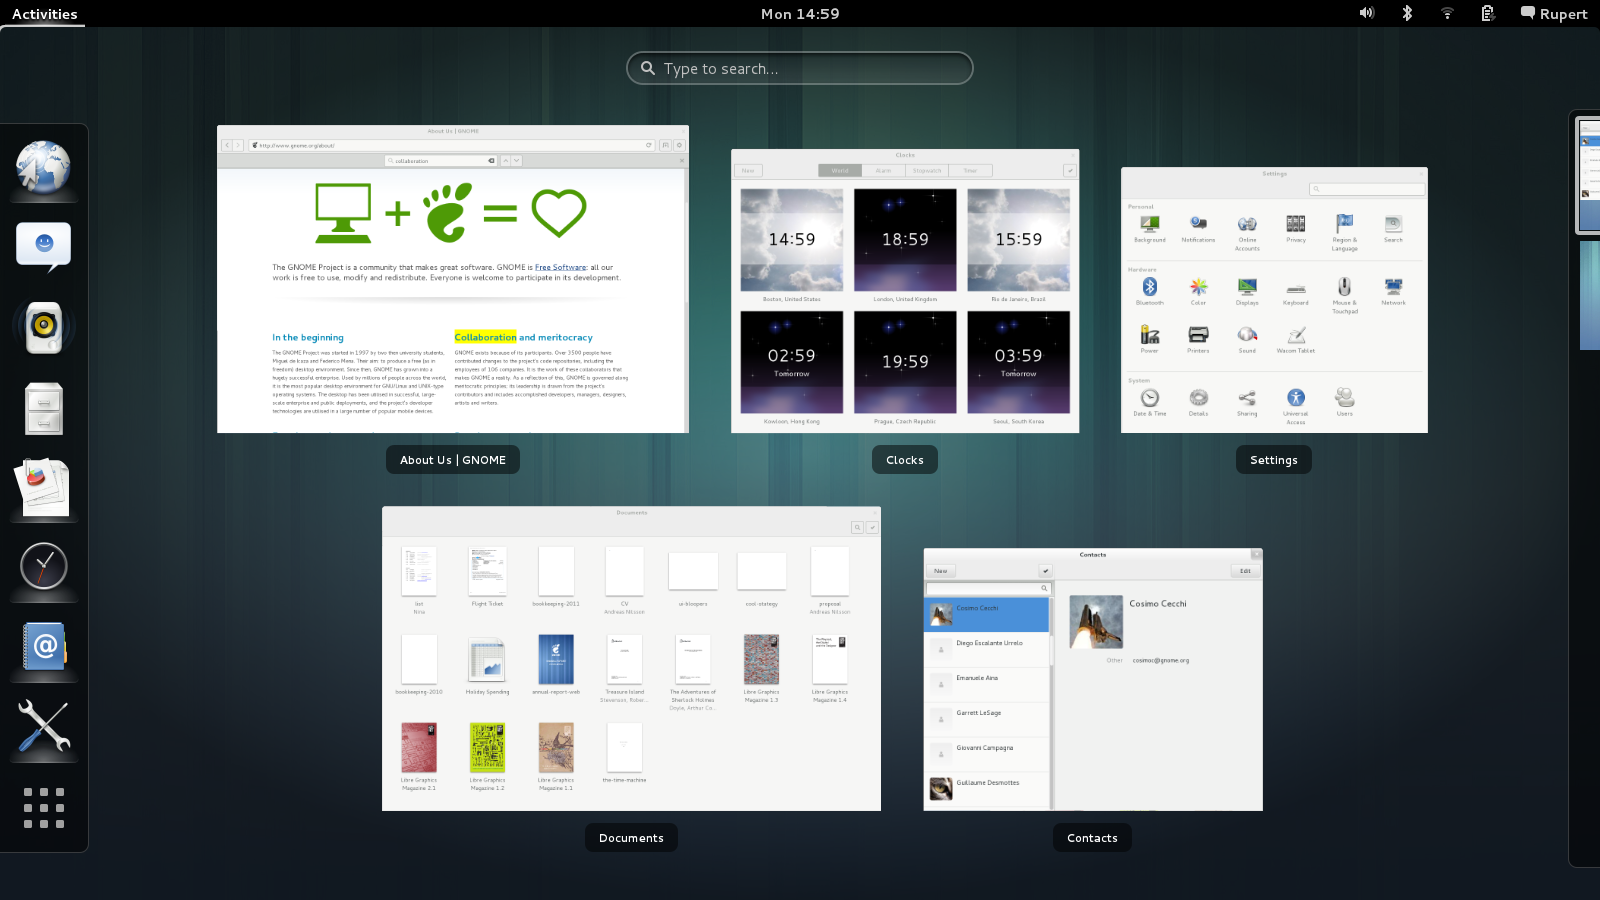
\includegraphics[width=11cm]{images/gui-example.png}
    \caption{Příklad grafického uživatelského rozhraní (TODO: zdroj -- gnome-shell).}
\end{figure}

Na vývoj grafických uživatelských rozhraní má vliv mnoho aspektů mezi něž patří mimo jiné i způsob interakce člověka s počítačem. Už na začátku osmdesátých let se začali objevovat první polohovací zařízení, díky kterým se postupně eliminovaly nedostatky textových rozhraní---především jejich nemožná integrovatelnost mezi běžné uživatele. Tím vznikla základní podoba WIMP konceptu (\textit{Windows, Icons, Menus, Pointer}), která představuje základní rysy dnešních GUI.

Pojem \textit{grafické uživatelské rozhraní} bývá často používán výhradně pro označení rozhraní, které umožňuje uživatelům komunikovat s elektronickým zařízením (integrované např. v operačním systému). Tato definice je však nepřesná, protože neoznačuje systémy, které operují jako tzv. tenký klient. Tenký klient je typ zařízení nebo aplikace, jejíž funkčnost je závislá na jiném zařízení (serveru). Tyto aplikace slouží především pro prezentaci informací uživateli, zatímco zpracování a ukládání dat provádí server. Příkladem aplikace, která pracuje na tomto principu je Internetový prohlížeč.

\section{Webové uživatelské rozhraní}
\label{sec:wui}

Webové uživatelské rozhraní (anglicky \textit{Web-based User Interface}, zkráceně WUI) je typ grafického uživatelského rozhraní, které je součástí webových aplikací. Webová aplikace je typ programu, jehož funkce a nástroje jsou přístupné přes HTTP protokol. Interakce mezi uživatelem a programem je pak zajištěna webovým prohlížečem.

\begin{figure}[htbp]
    \centering
    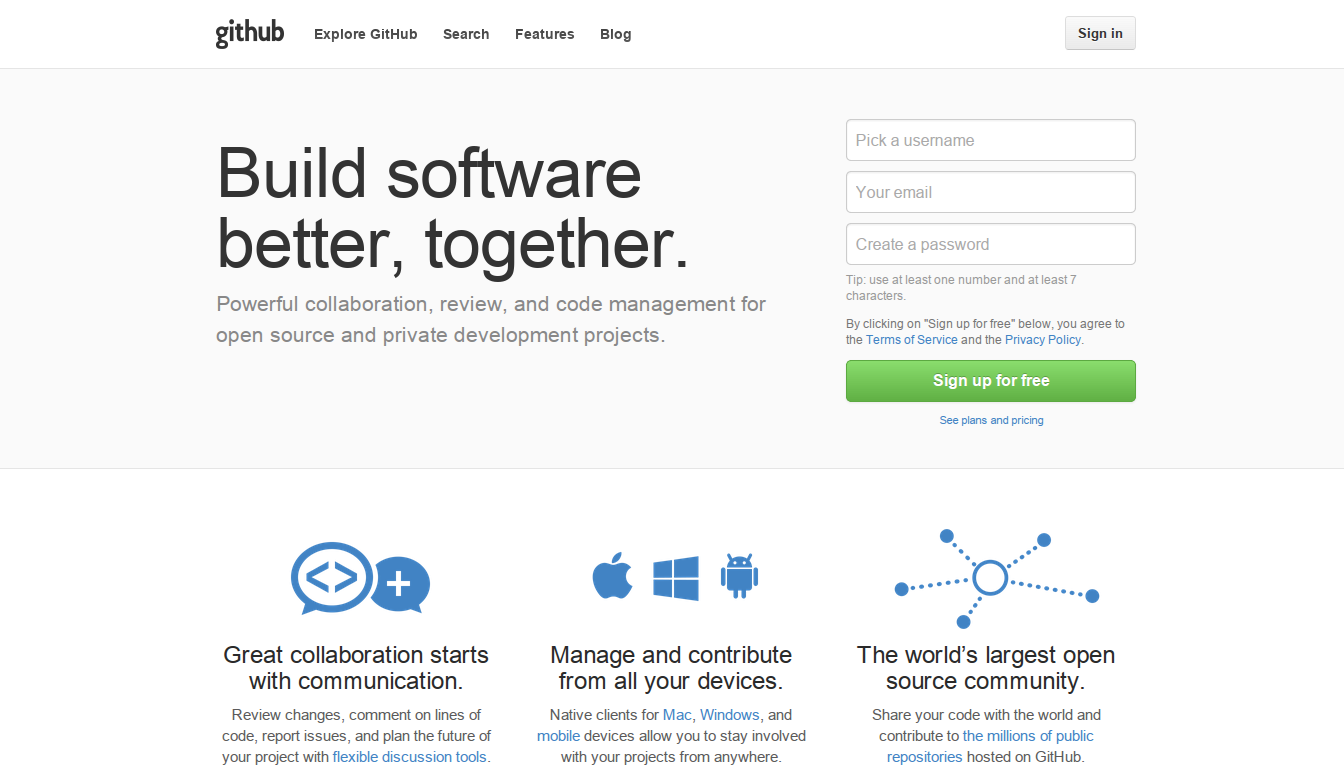
\includegraphics[width=11cm]{images/wui-example.png}
    \caption{Příklad webového uživatelského rozhraní (TODO: zdroj -- github.com).}
\end{figure}

Mezi hlavní výhody webových aplikací patří relativně jednoduchá udržovatelnost a flexibilita. Tyto vlastnosti jsou dány povahou klient--server modelu. Jedná se o síťovou architekturu, která rozlišuje klienta (uživatele) a server (aplikaci). Klient--server model umožňuje vývojářům udržovat pouze jednu verzi aplikace, která je multiplatformní a často daleko bezpečnější a spolehlivější. Nevýhodou je nižší dostupnost a vyšší odezva, která je dána kvalitou síťového (Internetového) připojení.
